% Chương 4
\chapter{KẾT QUẢ} % Tên của chương

\label{Chapter4} % Để trích dẫn chương này ở chỗ nào đó trong bài, hãy sử dụng lệnh \ref{Chapter4}

\begin{figure}[h!]
	\centering
	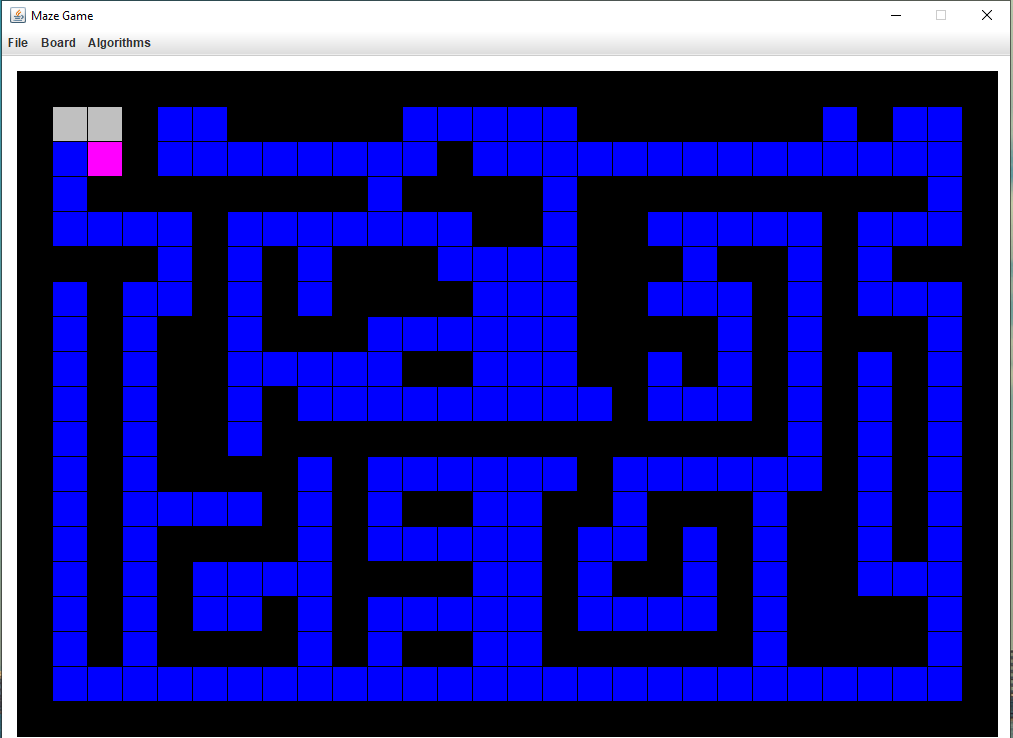
\includegraphics[width=0.4\textwidth]{
		Figures/figs/7.png
	}
	\caption[Trạng thái ban đầu]{
		Trạng thái ban đầu
	}
	\label{fig:hinh8}
\end{figure}

Với trạng thái bắt đầu là trạng thái ở hình trên, ta có kết quả thực hiện tương ứng với các thuật toán.

\newpage
\section{Kết quả thuật toán BFS}
\begin{figure}[h!]
	\centering
	\includegraphics[width=0.5\textwidth]{
		Figures/figs/BFS.jpg
	}
	\caption[Kết quả thuật toán BFS]{
		Kết quả thuật toán BFS
	}
	\label{fig:hinh11}
\end{figure}

Số bước đi = 4

Số phép toán đã thực hiện = 30

Thời gian tính toán = 0.015s


\newpage
\section{Kết quả thuật toán DFS}
\begin{figure}[h!]
	\centering
	\includegraphics[width=0.5\textwidth]{
		Figures/figs/DFS.jpg
	}
	\includegraphics[width=0.5\textwidth]{
		Figures/figs/DFS_2.jpg
	}
	\caption[Kết quả thuật toán DFS]{
		Kết quả thuật toán DFS
	}
	\label{fig:hinh12}
\end{figure}

%\begin{figure}[h!]
%	\centering
%	\includegraphics[width=0.5\textwidth]{
%		Figures/figs/DFS_2.jpg
%	}
%	\caption[Kết quả thuật toán DFS 2]{
%		Kết quả thuật toán DFS 2
%	}
%	\label{fig:hinh15}
%\end{figure}

%\newpage
Chi phí tối đa của thuật toán = 15

Số bước đi = 8

Số phép toán đã thực hiện = 3244

Thời gian tính toán = 0.047s



